\usetikzlibrary{decorations.pathmorphing}
\usetikzlibrary{decorations.markings}
\usetikzlibrary{decorations.pathmorphing}
\usetikzlibrary{arrows}
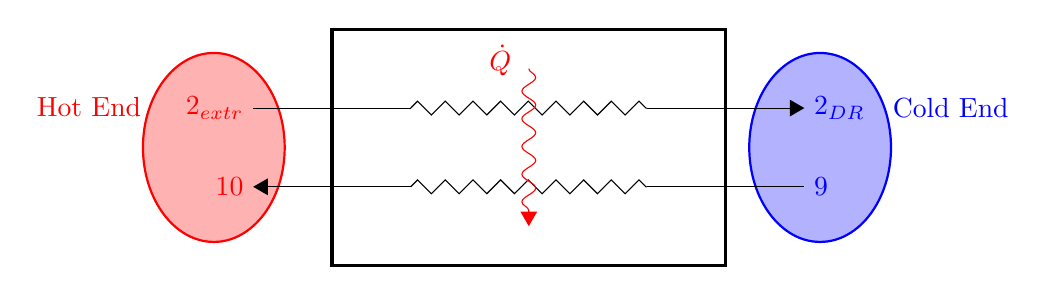
\begin{tikzpicture}[>=triangle 60]
% rectangle
\draw[very thick] (0,0) rectangle (5,3);
% cold end
\draw[fill=blue!30,draw=blue,thick] (6.2,1.5) ellipse (0.9 and 1.2);
\node[blue,right] at (7,2) {Cold\ End};
% hot end
\draw[fill=red!30,draw=red,thick] (-1.5,1.5) ellipse (0.9 and 1.2);
\node[red,left] at (-2.3,2.02) {Hot\ End};
% air line
\draw[]  (-1,2)--(1,2);
\draw[decorate,decoration=zigzag] (1,2)--(4,2);
\draw[->]  (4,2)--(6,2);
% flue gas linetriangle 60
\draw[<-]  (-1,1)--(1,1);
\draw[decorate,decoration=zigzag] (1,1)--(4,1);
\draw[]  (4,1)--(6,1);
%
\node[red,left] at (-1,2) {$2_{extr}$};
\node[red,left] at (-1,1) {$10$};
%
\node[blue,right] at (6,2) {$2_{DR}$};
\node[blue,right] at (6,1) {$9$};
% heat transfer
\draw[red, decorate,decoration={snake,post length=1.5mm}, ->] (2.5,2.5)--(2.5,0.5);
%\draw[red,<-]  (2.5,0.5)--(2.5,0.5);
\node[red,left] at (2.4,2.6) {$\dot{Q}$};
\end{tikzpicture}